% --
% mfcc

\section{Mel Frequency Cepstral Coefficients}\label{sec:signal_mfcc}
\thesisStateReady
Very commonly Mel Frequency Cepstral Coefficients (MFCC) are used as input features for neural network classifications tasks in speech recognition.
It is described why MFCCs are good features for speech signals, how they are calculated in detail, how they can be enhanced and in which way they can be visualized to understand them better.


% --
% idea

\subsection{The Idea}
The processing scheme of MFCCs is as following:
Raw audio samples are transformed into the frequency domain with the Short-Time Fourier Transform (STFT).
Afterwards the power spectrum of the STFT is segmented in frequency bands (along the frequency dimension) done by a filter bank.
The filter bands are spaced in equidistant Mel frequencies, where Mel frequencies represent the non-linear relationship between the Mel and frequency scale.
The Mel scale was developed in psycho-acoustic experiments, where researchers found out, that high frequency sounds (above approximately \SI{500}{\hertz}) are perceived lower than they actual are in the musical sense of pitch.
In the musical sense, a pitch interval of an octave is the doubling of the frequency of a fundamental frequency, but human hearing is different in the perception and frequency doubling does not necessarily double the perceived pitch.
As conclusion the Mel scale is suited human hearing perception of pitch and taking equidistant Mel bands is a reasonable approach.

Another important processing step is the logarithmic scaling of the power spectrum's value space, because humans perceive loudness in the logarithmic scale.
The last step is not that straight forward, but is a technique widely used in image processing called the Discrete Cosine Transform (DCT).
Note that the DCT is some kind of decorrelation process to mix filter bands in different constellations together.

This processing steps seem rather complicated, but are in fact nothing else but consecutive steps of appropriate scaling and data compression.
In fact neural networks are able to handle large amounts of input features, but it is always preferable to minimize the input size, hence the model size and training time are decreased and therefore computations saved.


% --
% processing pipeline

\subsection{Processing Pipeline in detail}\label{sec:signal_mfcc_pipeline}
The frequency spectrum is separated into filter bands through triangular window functions.
Those window functions are equidistantly placed onto the Mel scale and therefore give a varying number of frequency bins in the frequency scale of each window.
The lower frequency bands receive less frequency bins than the high frequency bands.
Sometimes the height of the triangular windows are scaled down so that the effect of unequal amounts frequency bin numbers is equalized, however high frequencies carry less energy and therefore this scaling is in most cases not needed, therefore all the triangular windows have their peak at the value $1$.
The Mel - Frequency relation can be approximated with:
% mel
\begin{equation}\label{eq:signal_mfcc_mel}
  m(f) = 2595 \cdot \log_{10} \left(1 + \frac{f}{700} \right) 
\end{equation}
where $m$ is the result in Mel scale as function of the frequency $f$.
The Mel scale plotted against the frequency scale is illustrated in \rfig{signal_mfcc_mel_scale}.
% mel fig
\begin{figure}[!ht]
  \centering
  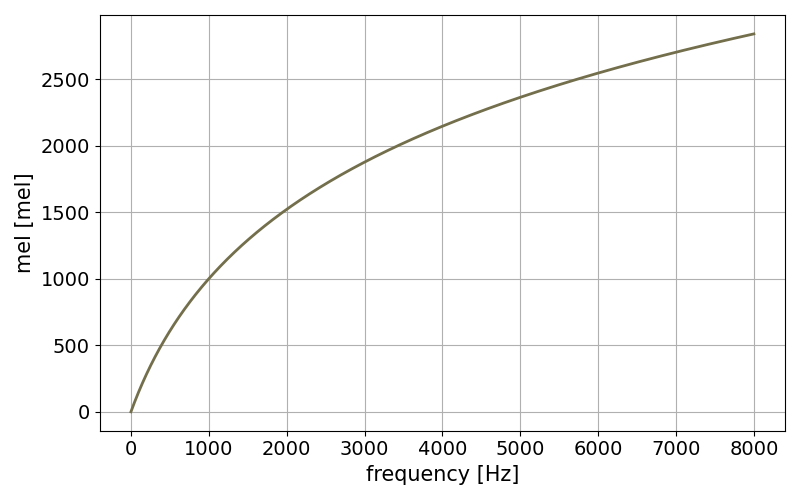
\includegraphics[width=0.40\textwidth]{./3_signal/figs/signal_mfcc_mel_scale}
  \caption{Mel scale as function of the frequency in a range of [0, \SI{16}{\kilo\hertz}].}
  \label{fig:signal_mfcc_mel_scale}
\end{figure}
\FloatBarrier
\noindent
The Mel and frequency window functions or equidistant Mel filter bands are shown in \rfig{filter_bands}.
\begin{figure}[!ht]
  \centering
  \subfigure[mel space]{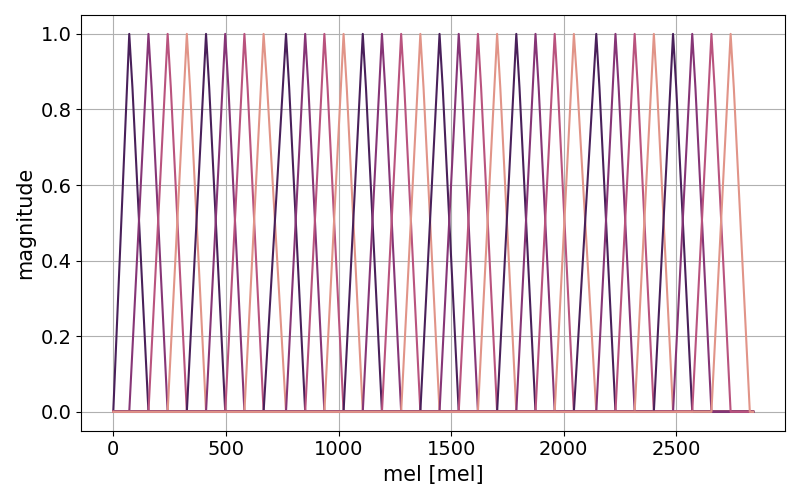
\includegraphics[width=0.40\textwidth]{./3_signal/figs/signal_mfcc_weights_mel}}
  \quad
  \subfigure[frequency space]{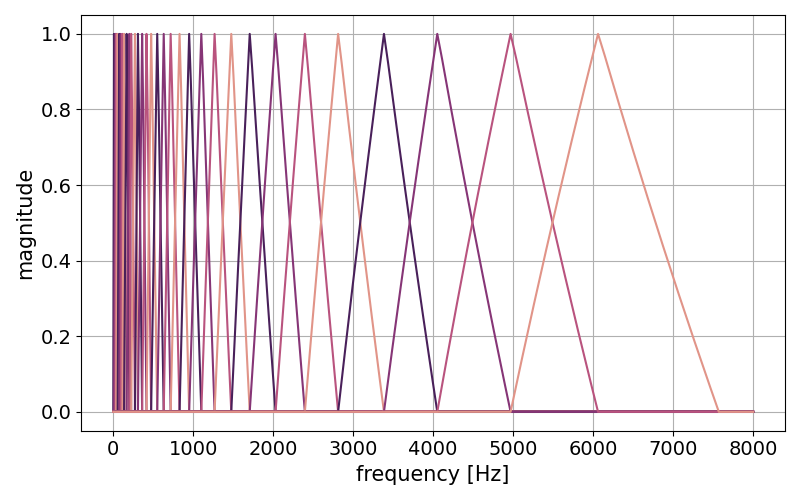
\includegraphics[width=0.40\textwidth]{./3_signal/figs/signal_mfcc_weights_f}}
  \caption{Equidistant Mel filter bands with a total number of 32 bands.}
  \label{fig:filter_bands}
\end{figure}
\FloatBarrier
\noindent
The creation of those filter bands is not described mathematically, because the graphical showcase is much more intuitive and easier to understand.
For further calculations, those filter bands are notated in a weight matrix called $W_m \in \R^{B \times N}$, where $B$ are the amount of used filter bands as rows in the matrix and $N$ the amount of frequency bins of the DFT transformed input signal as columns.

% dct
The DCT is very similar to the Fourier transform and projects the input signal to a set of orthogonal basis functions, however the transformed signal is real valued only instead of complex valued.
Different types of DCTs formulations exists, but most commonly the \enquote{type 2} DCT is used and can be calculated as:
% dct
\begin{equation}\label{eq:signal_mfcc_dct}
  X[c] = \sum_{n=0}^{N-1} x[n] \, \cos{\left[ \frac{\pi}{N} \left( n + \frac{1}{2} \right) c \right]}
\end{equation}
with $c$ as DCT coefficient index and $n$ as sample index of a signal with total length of $N$.
This can be conveniently written in matrix notation with a total number of $C$ DCT coefficients:
% dct matrix
\begin{equation}\label{eq:signal_mfcc_dct_matrix}
  X =  x \, \mathcal{D} \quad \mathrm{with} \quad \mathcal{D}[n, c] = \cos{\left[ \frac{\pi}{N} \left( n + \frac{1}{2} \right) c  \right]}, 
  \quad n, c = (0, 1 \dots N - 1), (0, 1 \dots C) 
\end{equation}
with $\mathcal{D} \in \R^{N \times C}$ as DCT matrix and input signal $x \in \R^N$ which gives the transformed signal $X \in \R^C$
The DCT basis functions illustrated in a matrix in two different color schemes are shown in \rfig{signal_mfcc_dct}.
\begin{figure}[!ht]
  \centering
  \subfigure[DCT with continuous color scheme]{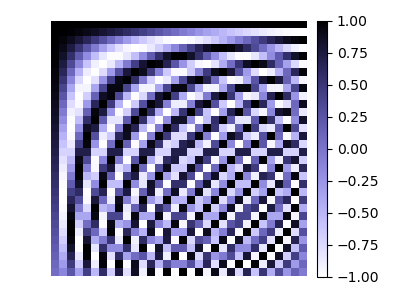
\includegraphics[width=0.35\textwidth]{./3_signal/figs/signal_mfcc_dct}}
  \quad
  \subfigure[DCT with diverging color scheme]{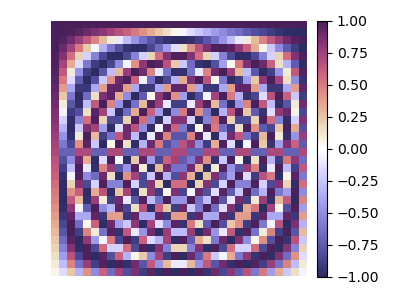
\includegraphics[width=0.35\textwidth]{./3_signal/figs/signal_mfcc_dct-div}}
  \caption{DCT matrix with 32 basis functions illustrated with a continuous and a diverging color scheme.}
  \label{fig:signal_mfcc_dct}
\end{figure}
\FloatBarrier
\noindent
The MFCCs $U \in R^{M \times C}$ are calculated from the log scaled power spectrum of the STFT $\tilde{X} \in \C^{M \times K}$ computed in \req{signal_spec_stft_matrix}, the filter band weights collected in the matrix $W_m \in \R^{B \times K}$ and transformed with the DCT matrix $\mathcal{D} \in R^{B \times C}$ as following:
\begin{equation}\label{eq:signal_mfcc_mfcc}
    U = \log{ \left[ \, \abs{\tilde{X}}^2 \, W_m^T \, \right] } \, \mathcal{D}.
\end{equation}
Note that the rows represent all shifts with the hop size and the columns are the individual cepstral coefficients of $U$.
The parameters to choose from are therefore the amount of filter bands $B$ and the amount of cepstral coefficients $C$.

Another important aspect is the visualization of MFCC features.
MFCCs computed as shown above, are not well intended for visualizations, because their individual coefficients value space differs strongly from each other.
For example the first coefficient equals a summation of all filter bands of the spectrogram and is therefore some kind of energy measure, while the other coefficients are different weighted sum combinations of the filter bands.
Further the most of the signal energy is located in the lower frequency bands, which impacts the value space of the coefficients with strongly weighted low frequency bands.
The differences in the value space leads to a problem in the visualization with a linear color scheme, so that some coefficients changes cannot be shown appropriately.
A solution to this problem is to normalize the feature vectors over each frame dimension with the infinity norm as:
% frame based normalization
\begin{equation}\label{eq:signal_mfcc_norm}
  \hat{U}[m, c] = \frac{U[m, c]}{\norm{u_c[m]}_\infty} \quad \forall m, c = (1, \dots, M), (1, \dots, C)
\end{equation}
where $m$ is again the frame (time) index, $c$ the individual MFCC coefficient and $u_c[m]$ the individual MFCC coefficient vector over all frames.
This equation gives a value space between $[0, 1]$ for each feature vector $u_c[m]$.

A visualization of MFCC features with 32 filter bands and 32 cepstral coefficients with frame based normalization of each coefficient is shown in \rfig{signal_mfcc_showcase_mfcc32}.
\begin{figure}[!ht]
  \centering
    \subfigure[left]{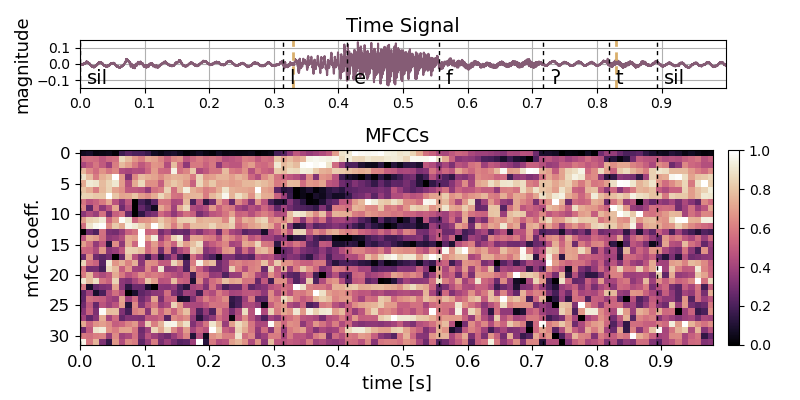
\includegraphics[width=0.45\textwidth]{./3_signal/figs/signal_mfcc_showcase_mfcc32_left0}}
    \subfigure[right]{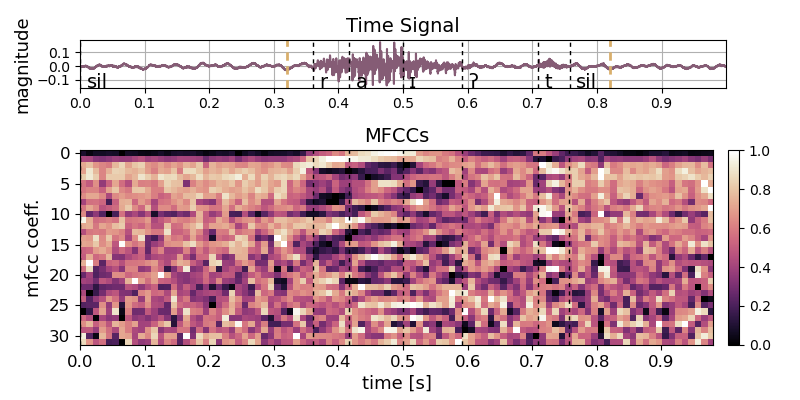
\includegraphics[width=0.45\textwidth]{./3_signal/figs/signal_mfcc_showcase_mfcc32_right0}}
    \subfigure[up]{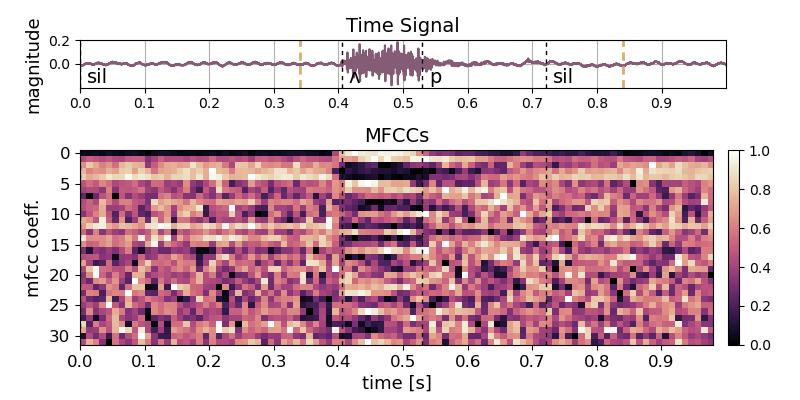
\includegraphics[width=0.45\textwidth]{./3_signal/figs/signal_mfcc_showcase_mfcc32_up0}}
    \subfigure[down]{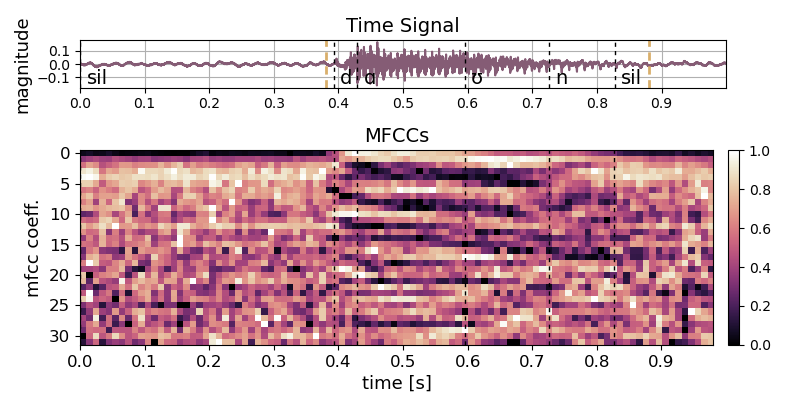
\includegraphics[width=0.45\textwidth]{./3_signal/figs/signal_mfcc_showcase_mfcc32_down0}}
    \subfigure[go]{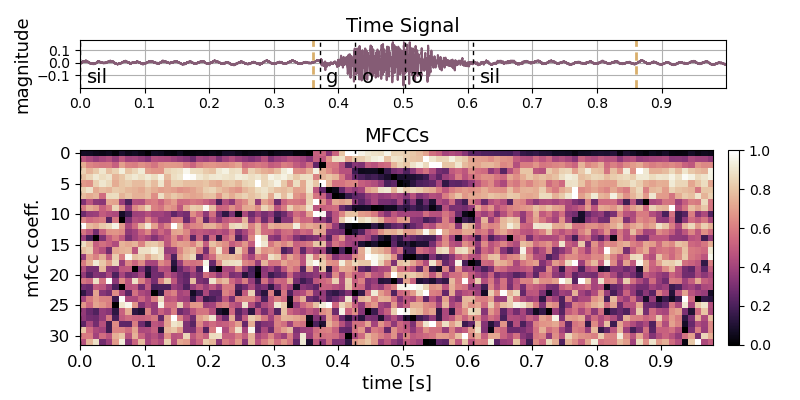
\includegraphics[width=0.45\textwidth]{./3_signal/figs/signal_mfcc_showcase_mfcc32_go0}}
  \caption{MFCC with 32 filter bands and 32 cepstral coefficients visualized with frame-based normalization.}
  \label{fig:signal_mfcc_showcase_mfcc32}
\end{figure}
\FloatBarrier
\noindent
The frame based normalization is an interesting aspect to improve the visualization of the MFCC features, however it can be critical. 
A normalization that operates only in one dimension changes important structures within the feature space and it cannot be answered yet if this is a problem for neural networks or degrades the classification performance.
One more research question arises here: Is it possible to use frame based normalized MFCC features as inputs to neural networks and what are the results to the accuracy and training of the models.


% --
% enhancement

\subsection{MFCC Feature Usage and Enhancement}\label{sec:signal_mfcc_enhancement}
After the MFCCs are computed with the choice of filter bands $B$ and cepstral coefficients $C$, they can already be used as input features for neural networks.
The question arises, whether feature enhancement can improve the performance in classification.
The best practice, used in many papers, is to apply $B=32$, $C=12$, compute derivatives of those 12 MFCC coefficients named as deltas (first derivative regarding the frame dimension) and double deltas (second derivative) and add energy vectors of the 12 coefficients and each one of the deltas.
The deltas are simply computed as frame $m$ difference of the MFCCs with:
\begin{equation}\label{eq:signal_mfcc_delta}
  \Delta u_i[m] = \frac{u_i[m - 1] + u_i[m + 1]}{2}
\end{equation}
where $u_i \R^M$ is the i-th MFCC coefficient vector and $m$ the frame index.
Note that the computation of the deltas at the edges $m=0$ and $m=M$ is not possible and the same value is obtained from the neighbor at this specific locations.
The second derivative of MFCC features, known as double deltas, are the frame differences of the deltas and in the same way computed as in \req{signal_mfcc_delta}.
Another enhancement is the computation of an energy feature vector of the MFCCs with:
\begin{equation}
  e[m] = u[m] \, u[m]^T 
\end{equation}
where $u[m] \in \R^C$ is the MFCC feature vector of frame $m$.
The same energy computation may also be applied to the deltas and double deltas each.
The MFCCs, their deltas, double deltas and energy vectors can simply be stacked at top of each other and used as enhanced feature inputs to neural networks.
In this thesis the feature vectors are stacked as following:
\begin{enumerate}
    \item 12 MFCCs
    \item 1 Energy feature of the 12 MFCCs
    \item 12 Deltas
    \item 1 Energy feature of the 12 Deltas
    \item 12 Double Deltas
    \item 1 Energy feature of the 12 Double Deltas
\end{enumerate}
which sums up to a 39-dimensional feature vector, very commonly used in the literature.
Many papers do not explicitly explain how the 39 MFCCs are calculated in detail, in most cases however this constellation is applied.
The computation of 39 MFCCs are shown in \rfig{signal_mfcc_showcase_mfcc39}
\begin{figure}[!ht]
  \centering
    \subfigure[left]{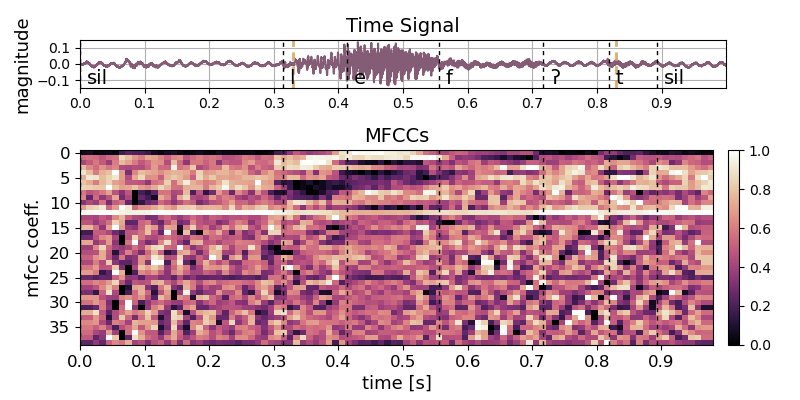
\includegraphics[width=0.45\textwidth]{./3_signal/figs/signal_mfcc_showcase_mfcc39_left0}}
    \subfigure[right]{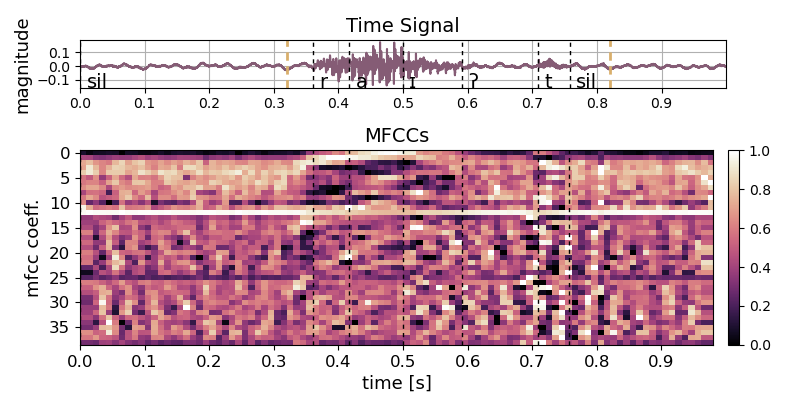
\includegraphics[width=0.45\textwidth]{./3_signal/figs/signal_mfcc_showcase_mfcc39_right0}}
    \subfigure[up]{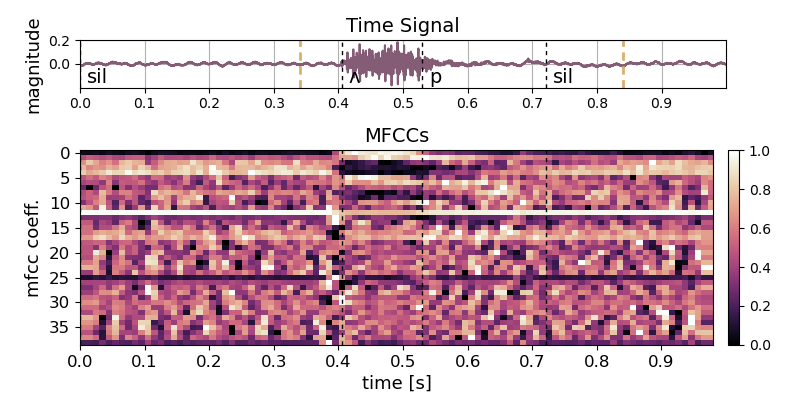
\includegraphics[width=0.45\textwidth]{./3_signal/figs/signal_mfcc_showcase_mfcc39_up0}}
    \subfigure[down]{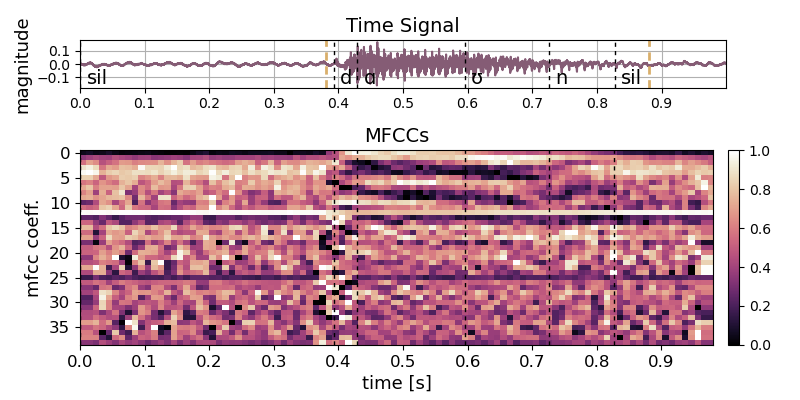
\includegraphics[width=0.45\textwidth]{./3_signal/figs/signal_mfcc_showcase_mfcc39_down0}}
    \subfigure[go]{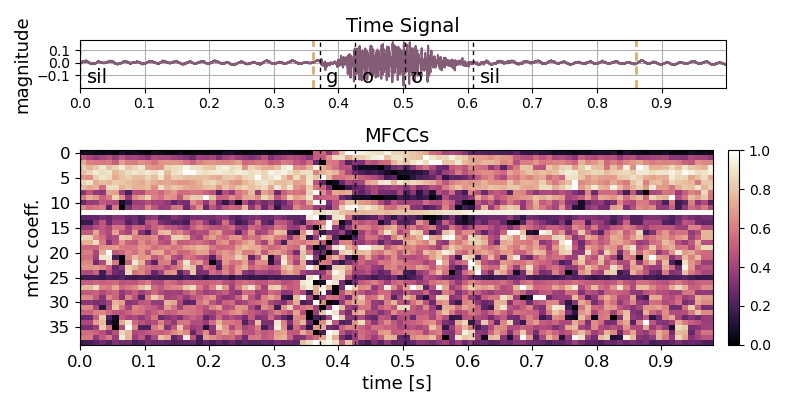
\includegraphics[width=0.45\textwidth]{./3_signal/figs/signal_mfcc_showcase_mfcc39_go0}}
  \caption{MFCC with 32 filter bands and 12 cepstral coefficients, deltas, double deltas and energy vector visualized with frame-based normalization.}
  \label{fig:signal_mfcc_showcase_mfcc39}
\end{figure}
\FloatBarrier
\noindent


% --
% energy consumption

\subsection{Energy consumption}
The energy consumption is evaluated on the amount of operations needed to process a \SI{1}{\second} time signal sampled with $f_s = \SI{16}{\kilo\hertz}$ to MFCC features.
All MFCC specific extraction details are collected in \rtab{signal_mfcc_extraction_params}.
\begin{table}[ht!]
\small
\begin{center}
\caption{Parameters for determining the computational complexity of the MFCC feature extraction process.}
\begin{tabular}{ M{7cm}  M{2.5cm} M{2.5cm}}
\toprule
\textbf{Parameter} & \textbf{Value} & \textbf{Sample Length} \\
\midrule
Length of a signal $n$ & \SI{1}{\second} & 16000 \\
Analytic window size $N$ & \SI{25}{\milli\second} & 400 \\
Hop size $h$ & \SI{10}{\milli\second} & 160\\
\midrule
Fourier coefficients $K$ & 400  & - \\
Number of filter bands $B$ & 32 & -\\
Number of cepstral coefficients $C$ & 12 & -\\
\bottomrule
\label{tab:signal_mfcc_extraction_params}
\end{tabular}
\end{center}
\vspace{-4mm}
\end{table}
\FloatBarrier
\noindent.
The amount of operations are the total number of additions and multiplications necessary to fulfill the process.
The major components of the MFCC are, as described in \rsec{signal_mfcc_pipeline} and summarized in \req{signal_mfcc_mfcc}, the transformation to the STFT, the weighting with the filter bands and the DCT transform.
The most costly component is of course the STFT, which again is composed of DFTs.
Note that the DFT uses complex multiplications and additions.
One complex multiplication equals to 4 real multiplication and 2 additions, so one complex multiplication consists of 6 operations.
For one complex addition, two real additions are necessary and equals therefore to 2 operations.
A general matrix multiplication with a vector $y = Ax$ where $A \in \R^{m \times n}$ and $x \in \R^n$ is composed of $m \cdot n$ multiplications and $m \cdot (n - 1)$ additions, where for simplicity the amount of additions is also assumed to be $m \cdot n$.

The amount of operations, denoted as $\mathcal{T(.)}$, for a trivial DFT transform with operator $\mathcal{F} \in \C^{N \times K}$ with $K$ Fourier coefficients on a windowed signal $x \in \R^N$ with sample length $N$ is:
% \begin{equation}
%   \mathcal{O}(x\mathcal{F}) = N \times K
% \end{equation}
\begin{equation}
  \mathcal{T}(x\mathcal{F}) = 6 (N K) + 2 (N K)
\end{equation}
and give for $N = K = 400$ the amount of operations $\mathcal{T}(x\mathcal{F}) = \SI{1.28}{\mega\ops}$ for a single DFT.
This of course are a lot of operations, luckily a more sophisticated Fourier transform can be applied with the Fast Fourier Transform (FFT) method, which gives a linear complexity and operations are calculated as:
\begin{equation}
  \mathcal{T}(x\mathcal{F}) = 6 (\mathcal{O}(N \cdot \log N)) + 2 (\mathcal{O}(N \cdot \log N))
\end{equation}
with $N = K = 400$.
The FFT has therefore roughly $\mathcal{T}(x\mathcal{F}) = \SI{20}{\kilo\ops}$ and is a huge improvement to the trivial method.
Further the interesting part of an DFT or FFT is only the half-band, because of the mirroring effect, which likewise may decrease the operations by half, so let the calculations be continued with Fourier coefficients of $K = 201$ of a half band and roughly $\SI{10}{\kilo\ops}$ per FFT.
The DFT is computed $M$ times, where $M$ is the total number of possible shifts calculated in \req{signal_spec_hop}, which gives with the evaluated parameters $M = 98$ frames.
So for the whole STFT $M$ is multiplied with the number of operations of each DFT, which give approximately $\mathcal{T}(\tilde{X}) = \SI{1}{\mega\ops}$.

The computation to the power spectrum and the log scaling are disregarded, so that two matrix multiplications remains:
$\abs{\tilde{X}}^2 \, W_m^T$ is a matrix multiplication of $\R^{M \times K}$ and $\R^{K \times B}$ which has $M K B$ real multiplications and approximately $M K B$ real additions, which give about $2 M K B = 2 \cdot 98 \cdot 201 \cdot 32 =  \SI{1.26}{\mega\ops}$.
The resulting band weighted STFT matrix $\R^{M \times B}$ is further multiplied with the DCT operator representing a matrix of $\R^{B \times C}$, that gives $2 M B C = 2 \cdot 98 \cdot 32 \cdot 12 = \SI{75}{\kilo\ops}$.
Altogether the matrix multiplications are approximately $\SI{1.26}{\mega\ops} + \SI{75}{\kilo\ops} = \SI{1.34}{\mega\ops}$.

The summary of the estimated operations are listed in \rtab{signal_mfcc_operations}.
% --
% mfcc operations
\begin{table}[ht!]
\begin{center}
\caption{Approximated number operations needed to transform a \SI{1}{s} time signal to MFCCs with parameters listed in \rtab{signal_mfcc_extraction_params}.}
\begin{tabular}{ M{6cm}  M{4cm}}
\toprule
\textbf{Process} & \textbf{Approximated Number of Operations} \\
\midrule
Power spectrum & \SI{2.71}{\mega\ops}\\
Weighting with equidistant Mel bands & \SI{1.26}{\mega\ops}\\
DCT transform of the weighted power spectrum & \SI{75}{\kilo\ops}\\
\midrule
\textbf{Sum} & \SI{4.05}{\mega\ops}\\
\bottomrule
\label{tab:signal_mfcc_operations}
\end{tabular}
\end{center}
\vspace{-4mm}
\end{table}
\FloatBarrier
\noindent



% delete me
%U = \log{ \left[ \, \abs{\tilde{X}}^2 \, W_m^T \, \right] } \, \mathcal{D}.


% --
% visualization

%\subsection{Visualization of MFCC features}\label{sec:signal_mfcc_visualization}


%To show this difference in value space in a negative example in practice, the MFCCs of the self-recorded speech command waveform \enquote{left0.wav} is shown in \rfig{left0_mfcc_only}.
% useless
% \begin{figure}[!ht]
%   \centering
%     \includegraphics[width=0.75\textwidth]{./3_signal/figs/signal_mfcc_left0_mfcc_only.png}
%   \caption{Bad visualisation of the 12 MFCCs features extracted from \enquote{left0.wav}.}
%   \label{fig:left0_mfcc_only}
% \end{figure}
% \FloatBarrier
% \noindent
% Not much structure of the MFCCs can be seen here, due to the vast value difference of the first coefficient. At least the first coefficient shows, where the center of signal energy is placed on the time scale, but other than that, this visualisation is worthless.
% Another very bad visualisation is shown by computing the 39 MFCC feature vectors (with Deltas, Double Deltas and Energies) in \rfig{left0_no_order}.

% \begin{figure}[!ht]
%   \centering
%     \includegraphics[width=0.75\textwidth]{./3_signal/figs/signal_mfcc_left0_no_order_norm0.png}
%   \caption{Very bad visualisation of 39 MFCC features extracted from \enquote{left0.wav}.}
%   \label{fig:left0_no_order}
% \end{figure}
% \FloatBarrier
% \noindent
% There appears an even greater gap of different value spaces and even less is seen.

% One solution is to show the features in different value groups. 
% For instance putting the first coefficient and its deltas is in one group, the other coefficients in another and their deltas and energies as well in own groups. 
% Now it is possible to observe some structure in the visualizations, with an example shown in \rfig{left0_order}.

% \begin{figure}[!ht]
%   \centering
%     \includegraphics[width=0.75\textwidth]{./3_signal/figs/signal_mfcc_left0_norm0.png}
%   \caption{Good visualisation of 39 MFCC features extracted from \enquote{left0.wav} with own value groupings.}
%   \label{fig:left0_order}
% \end{figure}
% \FloatBarrier
% \noindent
% Another way to improve the visualization is to normalize the feature vectors over each frame dimension with the infinity norm as:

% % frame normalisation
% \begin{equation}\label{eq:signal_mfcc_norm}
%   \hat{U}[m, l] = \frac{U[m, l]}{\norm{u_l[m]}_\infty}
% \end{equation}
% where $m$ is again the variable in frames, $l$ the individual MFCC coefficient and $u_l[m]$ the individual MFCC coefficient vector over all frames.
% This equation gives a value space between $[0, 1]$ for each feature vector $u_l[m]$.

% A visualization with frame normalization of the 39 MFCC feature vectors of \enquote{left0.wav} is shown in \rfig{left0_order},

% \begin{figure}[!ht]
%   \centering
%     \includegraphics[width=0.75\textwidth]{./3_signal/figs/signal_mfcc_left0_no_order_norm1.png}
%   \caption{Normalization of 39 MFCC features extracted from \enquote{left0.wav}.}
%   \label{fig:left0_no_order_norm1}
% \end{figure}
% \FloatBarrier
% \noindent
% or in an even better one shown in \rfig{left0_order_norm1}.

% \begin{figure}[!ht]
%   \centering
%     \includegraphics[width=0.75\textwidth]{./3_signal/figs/signal_mfcc_left0_order_norm1.png}
%   \caption{Normalisation of 39 MFCC features extracted from \enquote{left0.wav} with groups.}
%   \label{fig:left0_order_norm1}
% \end{figure}
% \FloatBarrier
% \noindent
